% =====================================================================
%  Free-history timescape: a data-driven void history reconciles the
%  supernova--BAO--CMB geometry but does not resolve the Hubble tension.
%
%  Paper 2+3 (combined) of the free-history timescape program.
%  DRAFT for arXiv (astro-ph.CO / gr-qc). Compile: pdflatex x2.
%  Class: revtex4-2 (matches paper 1, timescape-hubble-tension.tex).
%
%  >>> BEFORE SUBMITTING <<<
%   (1) Affiliation is final: "Independent Researcher" (no institutional affiliation).
%   (2) All arXiv ids machine-verified 2026-07-10 against live arXiv via the
%       committed verify_bibliography.py (+ verify_new_citations.py for the
%       lit-review additions). Wiltshire2009review / WiegandBuchert2010 /
%       ShethvdW2004 / ClampittJain2015 / Wiltshire2024 / GinatFerreira2026 /
%       Rincon2024 and DESI2024 / DESIDR2 carry arXiv-only entries (no journal
%       volume/page asserted).
%   (3) astro-ph.CO/gr-qc need an endorsement for a first-time submitter.
% =====================================================================
\documentclass[aps,prd,twocolumn,nofootinbib,superscriptaddress,floatfix]{revtex4-2}
\usepackage{amsmath,amssymb}
\usepackage{graphicx}
\usepackage{booktabs}
\usepackage{hyperref}
\hypersetup{colorlinks=true,linkcolor=blue,citecolor=blue,urlcolor=blue,
  pdftitle={Free-history timescape: a data-driven void history reconciles the
  supernova-BAO-CMB geometry but does not resolve the Hubble tension},
  pdfauthor={Viacheslav Zhygulin}}

\newcommand{\Ho}{H_{0}}
\newcommand{\Hbaro}{\bar H_{0}}
\newcommand{\fvo}{f_{v0}}
\newcommand{\fv}{f_{v}}
\newcommand{\fvz}{f_{v}(z)}
\newcommand{\kmsmpc}{\,\mathrm{km\,s^{-1}\,Mpc^{-1}}}
\newcommand{\Lcdm}{\Lambda\mathrm{CDM}}
\newcommand{\dBIC}{\Delta\mathrm{BIC}}
\newcommand{\rd}{r_{d}}
\newcommand{\bpred}{b_{\mathrm{pred}}}
\newcommand{\breq}{b_{\mathrm{req}}}
\newcommand{\Emax}{E_{\max}}
\newcommand{\gdress}{g_{\mathrm{dress}}}
\newcommand{\hmpc}{\,h^{-1}\mathrm{Mpc}}
% Defensive: any unresolved value would surface as a visible tag.
\newcommand{\todo}[1]{\textbf{[TODO: #1]}}

\begin{document}

\title{Free-history timescape: a data-driven void history reconciles the
supernova--BAO--CMB geometry but does not resolve the Hubble tension}

\author{Viacheslav Zhygulin}
\email{s.zhygulin@gmail.com}
\affiliation{Independent Researcher}
\date{\today}

\begin{abstract}
Paper~I showed that the timescape cosmology's one-parameter tracker closure cannot
jointly fit type~Ia supernovae (SNe), baryon acoustic oscillations (BAO), and the
cosmic microwave background (CMB) acoustic scale: the SNe pull the present void
fraction to $\fvo\simeq0.85$ while BAO$+$CMB demand $\simeq0.64$ (a
$4.8$--$6.6\sigma$ split), though a model-independent free-$E(z)$ check finds the
data consistent---the split is the tracker's rigidity, not a data conflict. Here we
free the void history $\fvz$, keeping the Buchert two-phase average and the
wall/void clock-rate dressing. The freed $\fvz$ reconciles Pantheon$+$, DESI BAO,
and the Planck acoustic scale at joint $\chi^2=1396.1$, below flat $\Lcdm$
($1402.2$) and far below the tracker ($1469.3$), at a plausible $\fvo=0.640$; the
amplitude split dissolves to $0.16\sigma$ (tracker: $6.5\sigma$), though this is a
single-amplitude check at fixed jointly-fit shape, not a proof of data consistency.
The reconciliation is covariance-dependent: under the cosmology-independent
covariance of Lane, Seifert et al.\ (FLRW-fiducial bias correction removed) the
supernova likelihood prefers $\Lcdm$ at every redshift cut ($\dBIC=+11$ to $+27$).
It is moreover kinematic---a backreaction target the Hubble diagram wants, violating
Buchert integrability---and fails four tests of independent physical \emph{character}
(availability, local-ladder bias, dynamical consistency, early-Universe
calibration), facets of one kinematic--dynamical gap: the required history declines
by $\times3.31$ over $0<z<2.33$ against an observed $\times1.16$ (a floor
theorem---level matched, shape unavailable); the predicted local bias is $+2.4\%$
against the $+8.4\%$ SH0ES requires (pre-registered PARTIAL, failing when the
observed catalog is forced in); enforced consistency collapses the three-phase
Buchert solve to the tracker, missing the geometry bar by $4953$; and the in-model
sound horizon $\rd=199.6$~Mpc ($+36\%$) drives the bare $\Hbaro$ to
$\sim\!32$--$40\kmsmpc$. The distance geometry reconciles, but the flexibility is
kinematic: consistent with Paper~I, free-history timescape does not resolve the
Hubble tension on present public data.
\end{abstract}

\maketitle

% =====================================================================
\section{Introduction}
\label{sec:intro}

The proposal that the apparent cosmic acceleration---and, by extension, the
Hubble tension---reflects the inhomogeneity of the late Universe rather than a
new energy component is the dark-energy-free inhomogeneity programme. The
timescape cosmology of Wiltshire~\cite{Wiltshire2007,Wiltshire2009,Wiltshire2009review}
is its most developed member: the present, void-dominated Universe is modelled as
a two-phase Buchert spatial average~\cite{Buchert2000,WiegandBuchert2010} of
spatially-flat ``walls'' (bound structures, where observers sit) and
negatively-curved ``voids,'' with a quasilocal clock-rate gradient (``dressing'')
so that a wall observer fitting Friedmann--Lema\^itre--Robertson--Walker (FLRW)
infers ``dressed'' parameters distinct from the volume-average ``bare'' ones.
Apparent acceleration follows without dark energy. The sharpest present challenge
to the $\Lcdm$ concordance model is the Hubble tension---the $\sim\!5\sigma$
discrepancy between the local distance-ladder value $\Ho\simeq73\kmsmpc$ and the
Planck$+\Lcdm$ early-Universe inference $\simeq67\kmsmpc$
\cite{Verde2023,Kamionkowski2022,CosmoVerse2025}. Recent Pantheon$+$ reanalyses
with a cosmology-independent covariance report strong Bayesian evidence for
timescape over $\Lcdm$~\cite{Lane2025,Seifert2024}, and Wiltshire has since argued
that the same void backreaction supplies the cosmological constant itself as an
averaging counterterm, requiring no separate dark-energy source~\cite{Wiltshire2024};
together these revive the question of whether the inhomogeneity framework also
addresses the Hubble tension.

This is the second paper of a three-paper arc. Paper~I~\cite{Paper1} subjected
the standard timescape \emph{tracker}---the one-parameter late-time attractor
that fixes the void-fraction history $\fvz$---to a uniform SN$+$BAO$+$CMB
harness and found that no single tracker fits the three geometry probes together:
the supernovae pull the present void fraction toward $\fvo\simeq0.85$ while the
BAO$+$CMB geometry demands $\fvo\simeq0.64$, a $4.8$--$6.6\sigma$ parameter split.
Crucially, a model-independent free-$E(z)$ spline fit to the same three datasets
matches $\Lcdm$: the data are \emph{not} internally contradictory. Paper~I
therefore diagnosed the tracker's one-parameter rigidity---not the timescape
mechanism, and not a genuine SN-versus-BAO data conflict---as the cause of the
combined-fit failure.

The present paper asks the immediate follow-up question: \emph{is the timescape
mechanism right but its tracker closure wrong?} We free the void history $\fvz$
from the tracker attractor, retain the Buchert two-phase average and the
wall/void clock-rate dressing unchanged, and re-test the framework end to
end---first against the SN$+$BAO$+$CMB geometry, then against every deeper
physical requirement the reconciling history must satisfy.

We state the two-part answer up front, qualitatively; the numbers follow in the
body. \textbf{Part~I} (Sec.~\ref{sec:reconcile}): freeing $\fvz$ \emph{does}
reconcile the geometry---the freed history fits Pantheon$+$, DESI BAO, and the
Planck acoustic scale below flat $\Lcdm$ and far below the rigid tracker, at a
physically plausible present void fraction, and the SN-versus-BAO$+$CMB amplitude
split all but vanishes. Throughout we label this reconciliation \emph{kinematic}:
it is a well-defined target the Hubble diagram wants, but the forced history need
not satisfy the Buchert integrability conditions and is not, on its face, a
general-relativistic solution; it is moreover specific to the supernova covariance
adopted. \textbf{Part~II} (Sec.~\ref{sec:partii}) confronts that history with four
requirements of independent physical \emph{character}---is the reconciling history
observationally \emph{available}, does it \emph{bias} the local ladder as needed,
is it a dynamically \emph{consistent} solution, and is it early-Universe
\emph{calibratable}? These are facets of a single kinematic-versus-dynamical gap,
not four decorrelated lines of evidence. All four fail: the required steep
void-fraction decline is absent from the observed void population
(\emph{shape-unavailable}); the predicted local expansion-rate bias falls an order
of magnitude short of what SH0ES requires (a pre-registered PARTIAL that fails
outright when the observed catalog is forced in); enforcing dynamical consistency
collapses the three-phase Buchert solve back to the two-phase tracker
(\emph{closed}); and the model's own sound horizon is far too large, driving the
bare Hubble rate well below both canonical values (\emph{fails}). This is
\emph{reconciliation without resolution}, and it corroborates and sharpens
Paper~I's conclusion.

Every quantitative claim below traces to a committed analysis script and its
result file (Sec.~\ref{sec:avail}); each verdict is stated against a
pre-registered threshold quoted before the verdict.

% =====================================================================
\section{Free-history timescape framework}
\label{sec:framework}

We use only what is needed; the derivations are in
\cite{Wiltshire2007,Wiltshire2009,Duley2013} and the uniform harness in
\cite{Paper1}. The void volume fraction $\fv(t)$ grows to a present value $\fvo$
in a two-phase Buchert average of walls and voids
\cite{Buchert2000,WiegandBuchert2010}. The lapse
$\bar\gamma\equiv dt/d\tau_w$ relates volume-average time $t$ to wall proper time
$\tau_w$; in the late-time tracker solution the dressed and bare Hubble
parameters obey \cite[eq.~(B9)]{Wiltshire2009}
\begin{equation}
\Ho=\gdress(\fvo)\,\Hbaro,\qquad
\gdress(\fvo)=\frac{4\fvo^{2}+\fvo+4}{2(2+\fvo)},
\label{eq:dressed}
\end{equation}
with $\bar\gamma_0=\tfrac12(2+\fvo)$. The tracker is the \emph{one-parameter}
closure that fixes the entire history $\fvz$ from $\fvo$ alone, and has been
fitted to multiple probes at a low dressed $\Ho$~\cite{Leith2008,Nazer2015}. We
drop it: we
let $\fvz$ be a free function on a redshift grid, solve the dressed geometry
(luminosity and transverse-comoving distances, following the DNW13 machinery
\cite{Duley2013} and the dressed-distance implementation of~\cite{Dam2017}) for
each admissible history, and later confront the freed history with the observed
void population.

Freeing the history exposes a lapse-convention choice that the tracker hides. We
carry two readings. \emph{LA (algebraic)} evaluates the lapse from the
tracker-form combination $\tfrac12(2+\fv)$ node by node. \emph{LB (rate-ratio)}
builds the lapse from the local expansion-rate ratio, so it depends on the
history's slope $\fv'(z)$ and fixes a self-consistent $\bar\gamma_0$ by shooting.
LA is the primary reading; LB, together with the no-lapse control (V0), brackets
the required history as a lapse-reading systematic used in Part~II.

\emph{Solver validation gate.} The general (non-tracker) dressed-geometry solver
is a faithful superset of the validated tracker geometry: driven to the tracker
history it reproduces the tracker limit to a maximum fractional transverse-distance
error $\lesssim6.5\times10^{-8}$ and an SN $\chi^2=1391.545$ (matching the Paper~I
tracker value), the LB gate passes at joint tracker $\chi^2=1469.293$ against the
reference $1469.293$, and it exhibits the genuine non-FLRW signature
$dD_M/dz\neq D_H\equiv c/H(z)$, which collapses to equality only in the FLRW
limit. This is the load-bearing statement that the machinery is correct before
we ask what it prefers.

% =====================================================================
\section{Part~I: Geometric reconciliation}
\label{sec:reconcile}

All Part~I results are \emph{kinematic}: they establish that the timescape
mechanism, with its history freed, has enough shape freedom to fit the distance
geometry. Whether that shape is physically realised is the subject of Part~II.

\subsection{Data and harness}
\label{subsec:data}

We reuse Paper~I's uniform harness and pipeline validation~\cite{Paper1}. The
supernova data are the Pantheon$+$ release~\cite{Scolnic2022,Brout2022}; the
cosmology sample is the $N=1580$ SNe with $z_{\mathrm{HD}}>0.01$ that are not
Cepheid calibrators ($0.010<z<2.26$), analysed under the full public
statistical$+$systematic covariance with the absolute-magnitude/$\Ho$ offset
marginalised analytically (the supernova verdict has historically been sensitive
to the light-curve fitter~\cite{Smale2011}, which the uniform harness holds
fixed across models). The main joint fit reuses Paper~I's DR1 SN$+$BAO$+$CMB
harness for direct comparability with Paper~I; DESI DR2~\cite{DESIDR2,DESI2024} is
used as a cross-check (Sec.~\ref{subsec:ampsplit}) and throughout Part~II. The CMB
enters only through the Planck 2018 acoustic-scale point~\cite{Planck2018}. As in Paper~I, the sound-horizon ruler $\rd$ enters BAO$+$CMB
only through the distance amplitude, so the redshift \emph{shape}---and hence the
history $\fvz$---is independent of the $\rd$ calibration (a fact we exploit, and
whose limits we probe, in Sec.~\ref{subsec:soundhorizon}).

\subsection{The required void history (Probe~R)}
\label{subsec:probeR}

We fit the freed history jointly to SN$+$BAO$+$CMB and compare, on identical
data, against the model-independent free-$E(z)$ spline, evolving dark energy
($w_0w_a$CDM, the DESI-hinted thawing direction~\cite{DESI2024}), flat $\Lcdm$,
and the one-parameter tracker
(Table~\ref{tab:jointchi2}). The pre-registered thresholds
\cite{Paper1} are: \emph{reconciles} if joint $\chi^2\le1412.24$
($=\chi^2_{\Lcdm}(\mathrm{DR1})+10$); \emph{disfavoured} if $\le1427.24$;
\emph{amplitude-dead} if $\ge1469.29$ (the tracker value). Part~I is referenced to
the DR1 $\Lcdm$ baseline ($\chi^2_{\Lcdm}=1402.24$); Part~II's model-comparison
bars are referenced to the DR2 baseline ($\chi^2_{\Lcdm}=1399.81$). The
$w_0w_a$CDM comparison is pertinent because inhomogeneity can itself masquerade as
evolving dark energy: Ginat and Ferreira~\cite{GinatFerreira2026} show that clumped
matter surrounded by voids, small-scale backreaction, and large-scale curvature
each distort luminosity and angular-diameter distances into an apparent
evolving-$w$ signal. That is a generic light-propagation effect; the freed $\fvz$
tested here is a specific two-phase Buchert realisation of it, with a definite
present void fraction and clock-rate dressing, which we hold in Part~II to the
further dynamical and observational requirements a real backreaction history must
meet.

\begin{table}[t]
\caption{Joint SN$+$BAO$+$CMB fit, identical data and harness: minimum $\chi^2$
of each model. The freed history (headline row) fits below flat $\Lcdm$ and far
below the one-parameter tracker; only the model-independent free-$E(z)$ spline
does better. The pre-registered reconcile threshold is joint
$\chi^2\le1412.24$. Column $k$ is the fitted parameter count; column
$\chi^2-\chi^2_{\Lcdm}$ is the difference from the $\Lcdm$ row. Raw $\chi^2$ is
compared; no information-criterion preference is claimed. The free-history
improvement over $\Lcdm$ carries $4$ extra parameters and is not significant
(Wilks $p=0.19$ on DR1, $0.82$ on DR2; BIC favours $\Lcdm$, $\dBIC\sim+23$ DR1 /
$+28$ DR2). The Wilks $p$-values are approximate---$\Lcdm$ is not nested within the
freed-history family, so they are indicative rather than exact---and the BIC
comparison, which needs no nesting, is the load-bearing one and points
conservatively toward $\Lcdm$. The comparison establishes kinematic
shape-sufficiency, not statistical preference.}
\label{tab:jointchi2}
\begin{ruledtabular}
\begin{tabular}{lccc}
Model & $k$ & joint $\chi^2$ & $\chi^2-\chi^2_{\Lcdm}$\\
\colrule
free $E(z)$ spline (model-indep.)      & spline & $1391.85$ & $-10.39$\\
free-history TS ($\fvz$) \emph{[this work]} & $5$ & $1396.06$ & $-6.18$\\
$w_0w_a$CDM                            & $3$ & $1398.29$ & $-3.95$\\
flat $\Lcdm$                           & $1$ & $1402.24$ & $0$\\
timescape tracker (1-param)           & $1$ & $1469.29$ & $+67.06$\\
\end{tabular}
\end{ruledtabular}
\footnotesize A no-lapse control (V0) gives $\chi^2=1396.49$, confirming the
result is not an artifact of the lapse convention. Under the
cosmology-independent Pantheon$+$ covariance of Ref.~\cite{Seifert2024}
(FLRW-fiducial bias correction removed) the shape-sufficiency fails: the fixed
free-history exceeds best-fit $\Lcdm$ by $\Delta(-2\ln\mathcal{L})=+18/+24/+35$ at
$z_{\min}=0.055/0.033/0.010$ (all above the $+10$ threshold),
$\dBIC(\mathrm{FH}-\Lcdm)=+11.1/+17.0/+27.2$ (fixed-history $k_{\rm cosmo}=0$;
$+45.8/+52.3/+64.0$ under an SN-fitted-nodes upper bound); the tracker reproduces
Ref.~\cite{Seifert2024}'s $\dBIC(\mathrm{TS}-\Lcdm)=+4.9/+1.5/-0.5$
(\texttt{seifert\_covariance\_row.json}).
\end{table}

The freed history reaches joint $\chi^2=1396.06$, comfortably inside the
reconcile band and $6.18$ below flat $\Lcdm$; only the model-independent
free-$E(z)$ spline ($1391.85$) does better, and the rigid tracker ($1469.29$) is
$67$ worse. The preferred present void fraction is $\fvo=0.640$ (LA), a
physically plausible value, coincident with the BAO$+$CMB-preferred value of
Paper~I and with timescape's own Planck fits~\cite{Nazer2015}. The associated
Hubble rates are a dressed $\Ho=63.97\kmsmpc$ ($\gdress$ convention), a full-rate
dressed $67.65\kmsmpc$, and a global bare $\Hbaro=53.79\kmsmpc$. The
pre-registered \textbf{Verdict: RECONCILES} (mechanism flexible). On DESI DR2 the
free-history
fit is $\chi^2=1398.28$ versus $\Lcdm$ $1399.81$ ($\Delta=-1.53$, Wilks
$p=0.82$), still inside the reconcile band; under BIC, $\Lcdm$ is preferred in
both DR1 and DR2---consistent with reading the reconciliation as kinematic
sufficiency, not model preference.

The reconciliation is robust to the lapse convention. The LB (rate-ratio) sibling
fits at $\chi^2=1406.92$ ($\fvo=0.588$; $+4.68$ above $\Lcdm$, still inside the
reconcile band), and its four validation gates all pass. The required-history
nodes for all three lapse readings are collected in Table~\ref{tab:fvnodes}: LA is
the primary reading; LB and V0 bracket the systematic.

\begin{table}[t]
\caption{Required void-fraction history $f_v^{\mathrm{req}}(z)$ at the fit nodes,
for the three lapse readings, from the joint SN$+$BAO$+$CMB fit. The last column
is the LA $\Delta\chi^2\le1$ band. LA is the primary reading.}
\label{tab:fvnodes}
\begin{ruledtabular}
\begin{tabular}{ccccc}
$z$ & LA & LB & V0 & LA $\Delta\chi^2\!\le\!1$\\
\colrule
$0$    & $0.640$ & $0.588$ & $0.383$ & $[0.638,0.641]$\\
$0.3$  & $0.531$ & $0.497$ & $0.250$ & $[0.521,0.533]$\\
$0.7$  & $0.396$ & $0.385$ & $0.128$ & $[0.384,0.407]$\\
$1.3$  & $0.279$ & $0.250$ & $0.072$ & $[0.231,0.318]$\\
$2.33$ & $0.194$ & $0.121$ & $0.017$ & $[0.148,0.231]$\\
\end{tabular}
\end{ruledtabular}
\end{table}

\subsection{The amplitude split dissolves}
\label{subsec:ampsplit}

Paper~I's headline pathology was that the SN and BAO$+$CMB data, fitted through
the rigid tracker, demand different present void-fraction \emph{amplitudes}. We
repeat that split test with the history freed, on DESI DR2 (a free-history joint
refit fits at $\chi^2=1398.28$, $\fvo=0.636$, versus $\Lcdm$ $1399.81$ and the
tracker $1514.10$). Fitting a single amplitude $A$ to the SN sector and to the
BAO$+$CMB sector separately, and jointly, gives $A_{\mathrm{SN}}=0.6351$,
$A_{\mathrm{BAO+CMB}}=0.6363$, $A_{\mathrm{joint}}=0.6360$, with a joint
excess $\Delta\chi^2=0.027$---an amplitude split of $\boldsymbol{0.16\sigma}$.
The same statistic applied to the tracker as a sanity check is consistent with
Paper~I's split: $\fvo^{\mathrm{SN}}=0.853$ against
$\fvo^{\mathrm{BAO+CMB}}=0.636$, $\Delta\chi^2=42.85$, a
$\boldsymbol{6.5\sigma}$ split---a single-amplitude $\Delta\chi^2$ statistic
recovering the same $0.85$-versus-$0.64$ tension Paper~I established with a
profile-likelihood parameter shift. The split \emph{dissolves} once the history
shape is free.

The interpretation is exactly Paper~I's diagnosis, now demonstrated
constructively: the SN and BAO$+$CMB data ``want'' the \emph{same} amplitude once
the history is free to bend. The $0.85$-versus-$0.64$ split was the tracker
parametrisation's rigidity, not a data conflict. One caveat bounds the claim: the
free-history split constrains only the single overall amplitude $A$ with the
jointly-fit shape held fixed (the four extra shape degrees of freedom having
already absorbed the SN-versus-BAO$+$CMB tension), so the $0.16\sigma$
demonstrates that the tracker's rigidity is removable, not that the data are
intrinsically consistent under this model.

\subsection{Why this is only a kinematic reconciliation}
\label{subsec:kinematic}

The reconciliation of Secs.~\ref{subsec:probeR}--\ref{subsec:ampsplit} is a
statement about distance geometry, not about dynamics. The forced $\fvz$
\emph{violates the Buchert integrability condition}. For a genuine single-phase
two-scale GR solution the void curvature parameter
$\alpha^{2}=-k_v\,f_{vi}^{2/3}$ must be constant in bare time
(DNW13 Eq.~11~\cite{Duley2013}); on the tracker it is constant to the
$\sim\!2\times10^{-6}$ pipeline floor, whereas the forced required history drifts
by $\sim\!152\%$ across its interior (Sec.~\ref{subsec:dynamical}). The freed
history is therefore ``the backreaction the Hubble diagram wants''---a
well-defined kinematic \emph{target}, not a demonstrated general-relativistic
solution. The geometric reconciliation is moreover specific to the supernova
covariance: repeating the SN comparison under the cosmology-independent covariance
of Refs.~\cite{Lane2025,Seifert2024}---which removes the FLRW-fiducial bias
correction the timescape programme regards as circular---the fixed free-history is
disfavoured relative to $\Lcdm$ at every redshift cut
(Table~\ref{tab:jointchi2}, footnote), so the shape-sufficiency of
Sec.~\ref{subsec:probeR} is not robust to that choice. (The evaluation is
deliberately fixed-shape and conservatively counted: the nodes are held at their
Part~I values and charged zero SN-side parameters, so the free-history enters
with \emph{fewer} parameters than $\Lcdm$ and the disfavouring is a likelihood
gap, $-2\Delta\ln\mathcal{L}=+18$ to $+35$, not a parameter penalty. Refitting
the nodes under the covariance of Refs.~\cite{Lane2025,Seifert2024} would define
a \emph{different} kinematic target, whose Part~II tests would then require
their own run; the question posed here is whether the Part~I reconciling
history itself is covariance-robust, and it is not.) Part~II asks, at full detail, whether that target is available in the
sky, consistent as dynamics, and calibratable to the early Universe.

% =====================================================================
\section{Part~II: Does the reconciliation survive?}
\label{sec:partii}

We report the four Part~II tests at the same length and specificity as the
Part~I reconciliation. Each states its pre-registered threshold before its
verdict. All four fail; the honest negative result is the value of the paper. Every
headline number in both parts was reproduced by an independent adversarial
re-derivation against its pre-registered threshold, with the per-check records
committed alongside the code (Acknowledgments and Sec.~\ref{sec:avail}).

\subsection{Availability: is the required history in the sky?}
\label{subsec:availability}

The reconciling history is a \emph{prediction} about the void population: the
required $\fvz$ must decline steeply with redshift. Over $0<z<2.33$ the LA
required history declines by a total factor $\times3.31$
(Table~\ref{tab:decline}). We confront this with the \emph{observed} void volume
fraction, measured from the BOSS DR12 galaxy sample with a watershed/ZOBOV void
finder (Mao et al.\ 2017~\cite{Mao2017}), calibrated to the $z=0$ 2M$++$ field
\cite{Carrick2015} and cross-checked against the watershed filling-fraction
literature~\cite{Pan2012,Williams2024}. The measurement chain is insensitive to
the standard void observational systematics: the $z=0$ anchor is the
real-space-reconstructed 2M$++$ field; the $z>0$ route uses the growth
\emph{ratio}, in which the redshift-space--distortion boost cancels to first
order; the light-cone gradient across an individual void (its far wall seen
$\sim\!2\times10^{8}$~yr earlier) is $<0.2\%$ in the volume fraction; and
per-sightline propagation effects are bounded by Paper~I's line-of-sight nulls
($\lesssim 0.05$~mag RMS).

\begin{table*}[t]
\caption{Required versus observed void-fraction decline. $f_v^{\mathrm{req}}$ is
the LA required history (Table~\ref{tab:fvnodes}); $r_{\mathrm{req}}$ is its
pre-registered decline-ratio band $f_v(z)/f_v(0)$ (mapping forecast);
$f_v^{\mathrm{obs}}$ and $r_{\mathrm{obs}}$ are the BOSS DR12 below-mean
measurement at the required grid. The $z=0$ \emph{level} matches (observed
$0.643$ inside the required band $[0.614,0.672]$); it is the \emph{shape}
(decline) that is unavailable. The observed decline is flatter than the required
band at every node above zero. Total decline $z\!=\!0\!\to\!2.33$: required
$\times3.31$, observed $\times1.16$.}
\label{tab:decline}
\begin{ruledtabular}
\begin{tabular}{cccccl}
$z$ & $f_v^{\mathrm{req}}$ (LA) & $r_{\mathrm{req}}$ band & $f_v^{\mathrm{obs}}$ & $r_{\mathrm{obs}}$ & status\\
\colrule
$0$    & $0.640$ & --- (anchor)       & $0.643$ & --- (anchor) & LEVEL-PASS (band $[0.614,0.672]$)\\
$0.3$  & $0.531$ & $[0.812,0.836]$     & $0.623$ & $0.968$      & FAIL: observed flatter\\
$0.7$  & $0.396$ & $[0.599,0.637]$     & $0.601$ & $0.934$      & FAIL: observed flatter (gap $0.205$, $52\%$)\\
$1.3$  & $0.279$ & $[0.361,0.499]$     & $0.578$ & $0.898$      & FAIL (growth-extrap.): $r_{\mathrm{obs}}>r_{\mathrm{req}}^{\mathrm{hi}}$\\
$2.33$ & $0.194$ & $[0.231,0.363]$     & $0.555$ & $0.863$      & FAIL (growth-extrap.): $r_{\mathrm{obs}}>r_{\mathrm{req}}^{\mathrm{hi}}$\\
\end{tabular}
\end{ruledtabular}
\footnotesize Observed $f_v$ measured on the primary below-mean route at $z=0.3$
and $z=0.7$ (BOSS DR12, $R_s=4\hmpc$); the Rs-sensitivity band at $z=0.7$ is
$[0.560,0.654]$ across $R_s\in\{2,4,8\}\hmpc$, all $\ge0.5$ (floor holds). The
$z=1.3$ and $2.33$ observed entries are $\Lcdm$-growth extrapolations of the
$z\le0.7$ BOSS DR12 below-mean measurement (propagated with the validated $\Lcdm$
$D(z)$ growth ratio), not direct measurements; at both nodes the observed ratio
exceeds the required-hi edge (pre-registered SHAPE test).
\end{table*}

\begin{figure}[t]
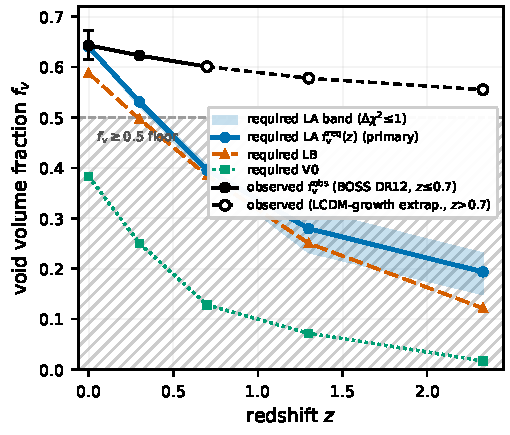
\includegraphics[width=\columnwidth]{fig_fv_required_vs_observed.pdf}
\caption{Required versus observed void volume fraction $f_v(z)$, all in the
bias-independent below-mean ($\delta<0$) definition. Solid blue: the primary LA
required history $f_v^{\mathrm{req}}(z)$ with its $\Delta\chi^2\!\le\!1$ band; the
LB and V0 lapse readings (dashed, dotted) bracket the systematic. Black: the
observed below-mean fraction---the $z=0$ 2M$++$ anchor (with its measured band)
and the $z\le0.7$ BOSS DR12 measurement as filled circles with a solid connector,
and the $z=1.3,2.33$ $\Lcdm$-growth extrapolations as open circles with a dashed
connector. The hatched region ($f_v<0.5$) is unreachable by any below-mean
population, whose volume fraction is bounded below by the $f_v\ge0.5$ floor
(floor theorem, Sec.~\ref{subsec:availability}). The
required history declines by $\times3.31$ over $0<z<2.33$ while the observed
population declines only $\times1.16$ and stays pinned above the floor; the
required curve crosses \emph{into} the excluded region between $z=0.3$ and
$z=0.7$ and lies well inside it at every higher node, so no admissible
below-mean population can supply its shape. Values are the committed availability
artifact \texttt{probes\_out/R2\_final.json} (verdict SHAPE-UNAVAILABLE), which
also backs Tables~\ref{tab:fvnodes} and~\ref{tab:decline}.}
\label{fig:fvhistory}
\end{figure}

The observed void fraction declines by a total factor of only $\times1.16$ over
the same range (Fig.~\ref{fig:fvhistory})---the population is far flatter than the
required history. At the
pivotal node $z=0.7$ the observed $f_v^{\mathrm{obs}}=0.601$ against a required
$0.396$, a gap of $0.205$ ($\sim\!52\%$ relative). This gap is not a statistical
undershoot but a \emph{floor theorem}: the below-mean void fraction---the volume
fraction with density below the cosmic mean---is at least half the volume
($\ge0.5$). This holds because the late-time volume-weighted density PDF is
right-skewed: for a lognormal field $P(\delta<\bar\delta)=\Phi(\sigma/2)\ge1/2$,
reaching $1/2$ only in the Gaussian (early-time) limit, and gravitational collapse
drives the skewness that way. Empirically the fraction is $\ge0.56$ across
$R_s\in\{2,4,8\}\hmpc$, giving the $z=0.7$ band $[0.560,0.654]$. The required
$f_v(0.7)=0.396$ lies \emph{below} the $0.5$ floor, so no admissible below-mean
population can reach it: the gap is unbridgeable by the definition, not a
large-significance undershoot. The
pre-registered SHAPE test declares the history
\emph{supplied} only if the observed decline ratio lies inside the required band
at every node; here the observed ratio exceeds the required-hi edge at every node
above zero. The $z=0$ \emph{level} matches (observed $0.643$ inside
$[0.614,0.672]$; required $\fvo=0.640$ passes), so it is specifically the
\emph{shape}, not the amplitude, that is unavailable.

\textbf{Verdict: SHAPE-UNAVAILABLE.} A fit-space corroboration
sharpens this: feeding the survey-measured history in with \emph{zero} free
parameters ($\fvz=f_v^{\mathrm{obs}}(z)$ fixed) gives a forced joint
$\chi^2=2845.6$ on DR2, missing the (one-fewer-parameter) BIC bar
\cite{KassRaftery1995} of $1407.2$ by $1438$; the miss is $>1400$ under every
covariance treatment tested (\texttt{verify\_forced\_joint\_fit.json}). The
theoretical two-phase $\fv$ is a
volume-average quantity that need not map onto any single void-finder definition;
accordingly the verdict is not that one definition falls short but that \emph{no}
tested observational definition supplies both the $z=0$ level and the decline. The
below-mean definition matches the level ($f_v(0)=0.643$ in the band
$[0.614,0.672]$) but is only $\times1.16$-flat, whereas a deep-void definition
($\delta<-0.3$) matches or exceeds the required $\times3.31$ decline but starts too
low ($f_v(0)\sim0.44$--$0.48$, failing the level)---no single void definition
occupies both corners. The $z=0$ level-pass is moreover specific to the LA reading:
LB ($\fvo=0.588$) and V0 ($0.383$) fall below the below-mean band, so availability
is worse under the lapse-reading systematic.

A commensurable and definition-free test is already within reach: the void-fraction
redshift evolution can be measured directly in the full-general-relativity
numerical-relativity watershed catalogs of Williams et al.~\cite{Williams2024}
already used here for the $z=0$ bracket, sidestepping the galaxy-survey definition
ambiguity entirely. On the observational side, newer and higher-redshift void
catalogs---DESIVAST from the DESI DR1 Bright Galaxy Survey~\cite{Rincon2024} and
the eBOSS void sample spanning $0.6<z<2.2$~\cite{Aubert2020}---can tighten the
$z=0$ level and extend the observed decline across the full required range; we
claim no such recomputation here, only that the measurement is sharpenable.

\subsection{The local expansion-rate bias $\bpred$}
\label{subsec:bpred}

For the model to resolve the Hubble tension \emph{as a local measurement bias},
its own two-scale structure must predict that a wall observer on the second rung
of the SH0ES distance ladder measures an apparent $\Ho$ high by a specific
amount. Define the target from the model's internal ladder-versus-global bare
Hubble offset,
\begin{equation}
\breq=\frac{\Hbaro^{\,\mathrm{anchored}}}{\Hbaro^{\,\mathrm{global}}}-1=+8.4\%
\quad(\breq=0.0842),
\label{eq:breq}
\end{equation}
which is the excess any local-bias mechanism must reproduce (the anchored fit
that fixes the numerator passes an $\Lcdm$ validation gate at
$\Ho=73.53\pm1.02\kmsmpc$, consistent with the SH0ES distance ladder
\cite{Riess2022}, recently re-anchored with HST Small Magellanic Cloud Cepheids
\cite{Breuval2024} and consolidated across estimators by the local distance-ladder
consensus~\cite{H0DN2025}). Equation~(\ref{eq:breq}) is a \emph{bare}-frame rate
ratio ($58.32/53.79-1$), and it is the \emph{smallest} of the admissible targets:
the corresponding dressed-frame ratio ($\sim\!73.5/64.0-1\approx0.15$) is nearly
twice as large, so reading $\breq$ in the dressed frame would only widen the
under-prediction found below. The verdict is therefore frame-robust.

\emph{The apparent-$\Ho$ window and the void-scale ceiling.} The tracker-form
combination
\begin{equation}
\Emax(\fvo)=\frac{3/2}{\gdress(\fvo)}-1,
\label{eq:emax}
\end{equation}
with $\gdress$ from Eq.~(\ref{eq:dressed}), is an algebraic identity that,
evaluated at Wiltshire's two published present void fractions, reproduces the
$17$--$22\%$ window as a consistency check (not an independent derivation):
$\Emax(0.76)=0.171$ and $\Emax(0.695)=0.220$ (validation gate a, matching the
literature window~\cite{Wiltshire2009,Wiltshire2009review,Wiltshire2013}). It is
used only for this window check and does \emph{not} give the ceiling adopted
below---at the fitted $\fvo=0.640$ it returns only $0.2615$. The void-scale
ceiling adopted below is a different quantity, the pure wall-observer clock
conversion
\begin{equation}
\Emax=\bar\gamma_0\,H_{v0}/H_{\mathrm{dress},0}-1=0.3365\quad(\text{LA};\ 0.208\ \text{LB}),
\end{equation}
evaluated on the fitted free history (gate b; this corrects an earlier
mislabeling of the volume-average $0.195$ as ``the maximum''). The ``maximum
apparent-$\Ho$ excess'' is thus a modelling choice spanning a factor $\sim\!3$
across conventions (tracker route $0.09$--$0.12$; volume-average $0.195$;
void-scale maximum $0.337$); we adopt the largest, model-favourable value, and the
FAILS verdict below is robust to the choice.

\emph{The SH0ES geometry dilutes the ceiling.} The second-rung Hubble-flow sample
does not sit at the void-scale maximum. The survey-averaged bias is
\begin{equation}
\bpred^{\,\mathrm{survey}}=\Emax\,\langle\varphi\rangle_{\mathrm{HF}}=0.0240,
\end{equation}
the void weight averaged over the $n_{\mathrm{HF}}=277$ Hubble-flow SNe
\emph{alone} ($\langle\varphi\rangle_{\mathrm{HF}}=0.0713$); the
$n_{\mathrm{calib}}=77$ calibrators
($\langle\varphi\rangle_{\mathrm{calib}}=0.994$) do \emph{not} enter, because the
SH0ES $M_B$ anchor is set by geometric Cepheid distances
(parallax/maser/detached-eclipsing-binary), unbiased by the local apparent rate.
This is a $14\times$ dilution of the ceiling $\Emax=0.3365$. Two bracketing
\emph{diagnostics} (neither is the primary): the differential
$\Emax(\langle\varphi\rangle_{\mathrm{calib}}-\langle\varphi\rangle_{\mathrm{HF}})=0.310$
is physically inapplicable (the calibrators sit deep in the void), and the
co-average over both populations, $0.092$, has no physical basis. The
lensing-\emph{physical} void rate (calibrated to stacked void lensing densities
\cite{ShethvdW2004,ClampittJain2015}) gives $\bpred^{\,\mathrm{phys}}=0.0158$, band
$[0.0150,0.0287]$. The entire admissible $\varphi$-band, $[0.0004,0.0720]$, lies
\emph{below} $\breq=0.0842$: a one-sided under-prediction.

\emph{Verdict against the pre-registered threshold.} The P3 threshold (P3 and P4
are Paper~I's pre-registered local-bias thresholds~\cite{Paper1}, on the bias
\emph{amplitude} and on its $z$-\emph{profile} respectively) is
$|\bpred-\breq|\le1\sigma\Rightarrow$ RESOLVES;
$\le2\sigma\Rightarrow$ PARTIAL; else FAILS. The decisive statement needs no
$\sigma$: the entire admissible $\varphi$-band $[0.0004,0.0720]$ lies below
$\breq=0.0842$, so the mechanism under-predicts the required survey-averaged bias
for \emph{every} admissible $\varphi$ (one-sided). Matching $\breq$ would require a
profile-decay scale $r_{\mathrm{hom}}^{\ast}=140\hmpc$, outside Wiltshire's
declared $[80,120]\hmpc$ band and beyond the $\sim\!137.5\hmpc$ 2M$++$ homogeneity
scale---where the density field is already homogeneous, so no apparent-$\Ho$ bump
can persist. Against the P3 tree the pre-registered significance is
$n\sigma_{\mathrm{prereg}}=1.57$ (PARTIAL), softened only by the wide
$\varphi$-shape \emph{theoretical} systematic, which the one-sided envelope shows
\emph{double-counts} $\sigma_\varphi$; the measurement-only
$n\sigma_{\mathrm{meas}}=4.16$ is the systematic-\emph{excluded} bound, reported
for completeness, not the basis of the verdict.

\emph{Catalog-forced cross-check (the symmetry rule).} Substituting the
\emph{observed} void population (Sec.~\ref{subsec:availability}) for the joint-fit
winner makes the mechanism fail harder, not softer: the anchored ceiling drops to
$\Emax^{\mathrm{obs}}=0.0657$ and $\bpred^{\,\mathrm{survey,obs}}=0.0047$, while
the forced global bare rate craters to $\Hbaro=50.8\kmsmpc$ (missing the BIC bar
by $1438$). The under-prediction ratio $\breq/\bpred$ is $17.9\times$ against the
fitted target and $68.1\times$ against the (larger) catalog-forced target.

\textbf{Verdict: PARTIAL} (pre-registered) \textbf{/ FAILS} (one-sided envelope and
catalog-forced). The pre-registered P3 outcome is PARTIAL, at $1.57\sigma$ (the
most-permissive of the registered readings; all lie below $2\sigma$, PARTIAL), and we
foreground it as the registered result. The family-level FAILS is the stronger
reading: it rests on the one-sided envelope---the entire admissible $\varphi$-band
lies below $\breq$---and on the catalog-forced test, in which the observed void
population under-predicts $\breq$ by $68\times$; it does not rest on relabeling the
$4.16\sigma$ measurement-only significance as robust. The envelope is decisive only
because it discards $\breq$'s own uncertainty, exactly the width the pre-registered
$1.57\sigma$ retains, so the two readings bracket the result rather than
contradict. Either way the predicted local bias is an order of magnitude below the
required $+8.4\%$---whether the void structure is fitted to the Hubble diagram or
supplied by the telescope---killing the local-bias resolution for this model family
regardless of Part~I's joint-fit quality.

\subsection{Dynamical consistency: is the required history a GR solution?}
\label{subsec:dynamical}

Section~\ref{subsec:kinematic} noted that the forced history violates Buchert
integrability; here (work package WP-B, the dynamical three-phase test) we quantify
it and make the honest attempt to \emph{restore}
consistency. The invariant $\alpha^{2}=-k_v\,f_{vi}^{2/3}$ (DNW13 Eq.~11
\cite{Duley2013}) must be constant in bare time for a genuine single-phase
two-scale GR solution. Its fractional drift across the interior of the forced
required history is $\sim\!152\%$. The magnitude is representation-dependent---the
five-node history under-determines $\fv''$, so the drift reads $\sim\!152\%$ on the
boundary-condition--robust interior window, $\sim\!1550\%$ over the full span, and
$\sim\!2150\%$ under the solver's monotone-PCHIP interpolation---but every reading
exceeds the tracker's $2\times10^{-6}$ pipeline floor by six-plus orders of
magnitude, so the integrability violation is robust to the representation. The
observed history drifts by $\sim\!5\times$ (span). An exact-analytic transcription
check drifts only at machine precision, so the drift is physical, not numerical.
\emph{No consistent single-phase Buchert model tracks either history.}

The honest attempt to make it consistent is a \emph{three-phase} Buchert solve
(shallow void, deep void, wall), which adds the dynamical degrees of freedom that
a single phase lacks. All four solver gates pass---G1 tracker-limit
($\mathrm{SN}\,\chi^2=1391.545$), G2 integrability, G3 lapse-limit
(agreement with $\tfrac12(2+\fv)$ to $4\times10^{-16}$), G4 numerics---and the
stage verdict is GO. But the best fit is \emph{degenerate}: with the four
constants pinned by the measured structure (the primary $k=0$ configuration), the
shallow void phase's amplitude drives to $\alpha_{s2}\to0$, i.e.\ the three-phase
model collapses to the two-phase empty-void tracker with a single genuine void of
fraction $f_{d0}\simeq0.27$. The tracking solution ``tracks'' only by becoming
the tracker.

The pre-registered geometry bar (DR2) is
$\chi^2\le\chi^2_{\Lcdm}(\mathrm{DR2})+\ln N\approx1407.2$. The zero-parameter ($k=0$)
forced-geometry prediction of the best three-phase constants gives a joint
$\chi^2=6360.2$, missing the bar by \textbf{4953}; a degeneracy check confirms
this equals the tracker prediction at $\fvo=f_{d0}=0.274$ to $0.02$ in $\chi^2$.
Even the never-a-claim \emph{constants-freed} diagnostic ceiling (the T1 ceiling of
Table~\ref{tab:wpn})---a different configuration, freeing the four constants the
theory pins by structure, in which
the \emph{deep}-phase amplitude collapses instead ($\alpha_{d2}\to7\times10^{-7}$
at $f_{d0}=0.022$)---misses the bar by $107$ ($\dBIC=+136$ versus $\Lcdm$).

\textbf{Verdict: CLOSED} (a theory-level close-out, not a numerical failure). The
required history is not a general-relativistic single-phase solution, and the
dynamical three-phase attempt to build one collapses back to the tracker it was
meant to generalise.

\subsection{The sound horizon: does it survive to the early Universe?}
\label{subsec:soundhorizon}

Part~I's fit borrowed the external drag-epoch sound horizon $\rd=147.09$~Mpc as a
ruler. WP-C (the sound-horizon work package) replaces that crutch with the model's
own bare-frame radiation-era physics (DNW13 machinery~\cite{Duley2013}) and asks
what $\rd$ free-history timescape actually predicts. The answer is
\begin{equation}
\rd^{\,\mathrm{in\text{-}model}}=199.6~\mathrm{Mpc},
\end{equation}
$+35.7\%$ above the external drag-epoch ruler $\rd=147.09$~Mpc (the in-model
decoupling-epoch radius is $r_{\mathrm{dec}}=195.9$~Mpc). The machinery
is validated: its $\Lcdm$ gate returns $r_\star=144.3$~Mpc and
$r_{\mathrm{drag}}=146.9$~Mpc, matching the expected values.

This in-model $\rd$ stands in tension with the timescape literature, which we own
rather than paper over. Fitting the CMB acoustic peaks within timescape, Nazer and
Wiltshire~\cite{Nazer2015} obtained an \emph{internally consistent} acoustic scale
at a dressed $\Ho\approx61\kmsmpc$; our bare-frame radiation-era treatment instead
returns $\rd=199.6$~Mpc and a bare rate far below that fit. The two are not yet
reconciled: our machinery is validated only on the $\Lcdm$ gate above, and the
disagreement lies in how the two calculations treat bare-frame recombination.
Reconciling them is an explicitly open task for the timescape programme---one it
already flags as unfinished, Seifert et al.~\cite{Seifert2024} noting that
calibration of the primordial sound speed and the BAO scale remains to be
done---rather than a settled result of this paper. We therefore report the in-model
$\rd$ as a self-consistency \emph{failure} of the freed history, not as a
determination of the timescape sound horizon.

Part~I's distance fit (Sec.~\ref{subsec:probeR}) is untouched by the in-model
$\rd$: its $\rd$-independence comes from the analytic $\alpha$-marginalization of
the BAO$+$CMB amplitude (Sec.~\ref{subsec:data}), which absorbs any overall ruler
rescaling---\emph{not} from the near-unity acoustic ratio. The in-model geometry
nonetheless disagrees with CMB early-Universe physics: although the acoustic ratio
$r_\star/r_{\mathrm{drag}}$ matches Planck to $0.03\%$ ($0.9816$ vs $0.9819$), the
in-model acoustic angle $\ell_A=218.9$ fails Planck's $301.7$ by $27\%$ ($291.9$
vs $301.7$ even when rescaled by the external $\rd$), with bare shift $R=1.11$ vs
$1.74$ and a BBN-$\eta$ baryon density $\omega_b=0.0186$ vs $0.0224$. The Part~I
CMB point therefore constrains only the redshift \emph{shape}, not agreement with
CMB early-Universe physics. But the \emph{absolute} Hubble rate is not
$\rd$-independent. With the
in-model $\rd$, the global bare rate drops from $\Hbaro=53.8$ to
$39.6\kmsmpc$, and the self-consistent fixed point is
$\Hbaro^{\ast}=32.4\kmsmpc$ (at $\rd^{\ast}=244.5$~Mpc), with the corresponding
dressed rates falling to $47.2$ ($\gdress$) and $49.9\kmsmpc$ (full-rate)---far
below both the reconciling band and SH0ES. Crucially, the failure is not an
artifact of the borrowed ruler: sound-horizon-independent $\Ho$ determinations,
which never invoke $\rd$---strong-lensing time delays~\cite{TDCOSMO2025},
water-megamaser geometric distances ($73.9\pm3.0\kmsmpc$)~\cite{Pesce2020}, and
gravitational-wave standard sirens~\cite{GWTC3siren}---all sit in the upper-$60$s
to mid-$70$s, far above the $\sim\!47$--$50\kmsmpc$ dressed rates that a self-consistent
in-model $\rd$ implies.

The pre-registered question is whether the Part~I \emph{absolute}-$\Ho$ claim
survives an in-model sound horizon; it does not
($R1_{\mathrm{survives}}=\mathrm{false}$, the pre-registered survival flag). As in
Paper~I, we distinguish resolution from
recasting: driving the bare Hubble rate \emph{below} both canonical values is a
recast of the tension, not a reconciliation near the local $\Ho$.

\textbf{Verdict: FAILS} (as an absolute-$\Ho$ claim). The model's own
early-Universe physics predicts a sound horizon $\sim\!36\%$ larger than the
ruler it had borrowed; forcing self-consistency collapses the bare Hubble rate to
$\sim\!32$--$40\kmsmpc$.

\subsection{Self-inflicted tensions (WP-N)}
\label{subsec:wpn}

Table~\ref{tab:wpn} aggregates the program's tension ledger (work package WP-N):
for each tension, the free-history (kinematic) status, whether it is
\emph{self-inflicted} by the
kinematic reconciliation, and the source artifact. The tally is $6$ YES
self-inflicted, $2$ partial, and $1$ target (the Hubble tension itself, which the
model exists to resolve). The synthesis is that the mechanism is CLOSED at every
level tested: the void geometry is shape-unavailable, the local SH0ES bias fails,
the dynamical three-phase consistency is closed, and the sound-horizon
absolute-$\Ho$ reconciliation fails.

\begin{table*}[t]
\caption{WP-N self-inflicted tensions of the free-history (kinematic) reading.
``Self-inflicted?'' marks tensions created \emph{by} the kinematic
reconciliation rather than inherited. Tally: $6$ YES, $2$ partial, $1$ target.
The growth/$S_8$ row (8) is structurally, not numerically, undefined: with no
perturbed metric the kinematic reading cannot even pose the $S_8$ question.}
\label{tab:wpn}
\begin{ruledtabular}
\begin{tabular}{p{0.185\textwidth}p{0.42\textwidth}p{0.07\textwidth}p{0.185\textwidth}}
Tension & Free-history (kinematic) status & Self-infl.? & Source\\
\colrule
Hubble (SH0ES vs.\ early) &
FAILS: $\bpred^{\mathrm{survey}}$ ceiling $0.0240$ $+$ physical $0.0158$ vs.\
$\breq=0.0842$; pre-registered $n\sigma_{\mathrm{prereg}}=1.57$ (PARTIAL), with the
systematic-\emph{excluded}, measurement-only $n\sigma=4.16$/$4.73$ (ceiling/physical)
reported for completeness, not as the verdict basis &
no (target) & \texttt{bpred\_survey\_averaged.json}\\
Required-vs-observed void shape (floor) &
SHAPE-UNAVAILABLE (obs decline $\times1.16$ vs.\ required $\times3.31$; floor
theorem) & YES & \texttt{R2\_final.json}\\
WP-B dynamical three-phase &
CLOSED: TRACKS degenerately but $k=0$ geometry misses BIC bar by $4953$; T1
ceiling misses by $107$ ($\dBIC=+136$) & YES & \texttt{threephase\_forced\_geometry.json}\\
Buchert integrability &
Not a single-phase GR solution: $\alpha^2$ drifts $\sim\!152\%$ (forced,
interior) / $\sim\!5\times$ (observed, span) vs.\ tracker $\sim\!2\times10^{-6}$ &
YES & \texttt{wpb\_integrability.json}\\
Void--wall contrast budget (two-sided) &
MARGINAL (field-mean $0.375$--$0.401$ $<$ required $0.474$ at $z=0$;
deep-void$+$wall $0.46$--$0.57$ reaches/exceeds it) & partial &
\texttt{contrast\_budget.json}\\
Q-budget (Stage 0) &
GATE=GO on empty/kinematic ceiling; physical budget $4$--$8\times$ short;
required contrast exceeds empty-Milne ceiling $\times1.36$ & YES &
\texttt{q\_budget.json}\\
Sound horizon / $\rd$ &
FAILS: in-model $\rd=199.6$~Mpc ($+36\%$); implied bare $\Hbaro$
$53.8\to\sim\!40$ (fixed point $32.4$) & YES & \texttt{wpc\_sound\_horizon.json}\\
Growth / $S_8$ &
UNDEFINED-IN-KINEMATIC-READING (no perturbed metric $\Rightarrow$ no growth
equation; measured $\sigma_m(z)$ is an input, not a prediction) & YES &
\texttt{NOTES\_growth.md}\\
$\bpred$ $z$-profile (P4) &
predicts local $\Ho$ bump decaying by $r_{\mathrm{hom}}\sim\!100\hmpc$;
$r_{\mathrm{hom}}^{\ast}=140$ to reach $\breq$ is outside declared $[80,120]$ and
beyond 2M$++$ homogeneity $\sim\!137.5$ & partial &
\texttt{bpred\_survey\_averaged.json}\\
\end{tabular}
\end{ruledtabular}
\end{table*}

The growth/$S_8$ row deserves separate note: it is
\emph{undefined-in-kinematic-reading}. The kinematic reconciliation has no
perturbed metric, so there is no growth equation on the averaged
background---$f\sigma_8$, RSD $\beta$, weak-lensing/$S_8$, cluster counts, and the
ISW are none of them rigorously defined. The measured
$\sigma_m(L=20\hmpc,z)$ count-in-cells amplitude ($A=0.444$, reduced
$\chi^2\approx0.22$) is an \emph{input}, not a prediction. This is a structural
boundary of the kinematic reading, not a computed defeat, and it is defined only
after the (closed) dynamical WP-B reading is built.

Two further ledger rows carry only a status token in Table~\ref{tab:wpn} and
warrant a sentence each, both having been run against pre-registered thresholds.
The \emph{void--wall contrast budget} asks whether real (lensing/2M$++$-measured)
void and wall contents can supply the fitted expansion contrast
$(H_v-H_w)/\langle H\rangle\simeq0.474$ at $z=0$; the pre-registered expectation was
an available contrast $0.25$--$0.45$ against a required $0.45$--$0.5$---a shortfall
expected but not presumed, with the explicit falsifier that a two-sided contrast
reaching the required band within measured densities would \emph{withdraw} the
tension. The self-consistent field-averaged two-sided contrast is $0.375$--$0.401$,
below the required $0.474$, but a deep-void-plus-overdense-wall combination reaches
$0.46$--$0.57$; neither refuted nor withdrawn, the pre-registered
\textbf{Verdict: MARGINAL} (two-sided). The \emph{Q-budget} Stage-0 pre-gate is an
order-of-magnitude go/no-go on the Buchert backreaction $Q$, registered as NO-GO
only if the most-permissive $Q$-ceiling falls below $Q_{\mathrm{req}}/3$ at every
$0.3\le z\le1.0$: the gate is \textbf{GO} on the empty/kinematic ceiling, but the
physical, lensing-capped budget runs $4$--$8\times$ short of $Q_{\mathrm{req}}$, and
the required contrast $(H_v-H_w)/\Hbaro=0.516$ at $z=0$ exceeds the empty-Milne
ceiling $0.379$ by $\times1.36$---unattainable by any physical void. Both rows
corroborate the availability and dynamical closures above rather than carrying a
verdict of their own.

% =====================================================================
\section{Discussion}
\label{sec:discussion}

The result is \emph{necessary but not sufficient}, made concrete. Paper~I's
diagnosis was correct: the SN-versus-BAO$+$CMB split is the tracker's one-parameter
rigidity, and freeing $\fvz$ removes it, reconciling the distance geometry below
$\Lcdm$ and collapsing the amplitude split from $6.5\sigma$ to $0.16\sigma$
(Sec.~\ref{sec:reconcile}). The reconciliation is nonetheless purely kinematic, and
the gap between kinematics and dynamics is the whole story. A distance fit
constrains only the redshift dependence of the expansion---the \emph{shape} of
$\fvz$---and shape freedom is cheap: a few extra spline nodes can bend a smooth
$E(z)$ onto the Hubble diagram. What a distance fit cannot see is whether that
shape is realised as a void population in the sky, whether it solves the Buchert
equations a real backreaction history must satisfy, whether it biases the local
ladder by the amount the tension needs, and whether it calibrates to the early
Universe. Each Part~II test interrogates one of these, and each is a facet of the
single fact that a kinematic target carries no dynamical or observational content
beyond the distances it was fitted to. The history is not present in the observed
void population (Sec.~\ref{subsec:availability}). It is not a single-phase GR
solution, and the dynamical three-phase attempt to build one collapses back to the
tracker (Sec.~\ref{subsec:dynamical}). Its in-model sound horizon is too large to
calibrate to the early Universe (Sec.~\ref{subsec:soundhorizon}). And it predicts a
local expansion-rate bias an order of magnitude too small
(Sec.~\ref{subsec:bpred}).

A \emph{positive} result would have required, jointly and specifically: an
observed void population steep enough to supply the $\times3.31$ decline (not the
observed $\times1.16$); a required history that is a single-phase
integrability-consistent Buchert solution (not one drifting $\sim\!152\%$ in
$\alpha^2$); and an in-model sound horizon near $147$~Mpc (not $199.6$). None of
these holds, and the local-bias prediction independently falls an order of
magnitude short. The distinction between resolution and recasting from Paper~I
recurs sharply here: even where the model can be pushed toward a lower absolute
Hubble rate, that is a recast of the tension---both canonical values reinterpreted
as biased relative to a lower global average---not a reconciliation near the local
$\Ho$.

The $S_8$/growth question is out of reach of the kinematic reading altogether: it
has no perturbed metric and hence no growth equation, so it cannot pose the
question, let alone answer it (Sec.~\ref{subsec:wpn}). We flag this as the
boundary of the kinematic reading, not as a computed defeat; a dynamical reading
that could pose it is exactly the (closed) three-phase construction of
Sec.~\ref{subsec:dynamical}.

% =====================================================================
\section{Conclusions}
\label{sec:concl}

Free-history timescape does not resolve the Hubble tension. Freeing the
void-fraction history from the one-parameter tracker removes the rigidity that
Paper~I identified and reconciles the SN$+$BAO$+$CMB distance geometry at joint
$\chi^2=1396.1$, below flat $\Lcdm$ ($1402.2$) and far below the tracker
($1469.3$), at a physically plausible $\fvo=0.640$, with the amplitude split
dissolving to $0.16\sigma$---though this last is a post-fit single-amplitude check
with the jointly-fit shape held fixed, not an independent proof of data
consistency. Even this geometric reconciliation is covariance-dependent: under the
cosmology-independent supernova covariance of Refs.~\cite{Lane2025,Seifert2024} the
fixed free-history is disfavoured relative to $\Lcdm$ at every redshift cut. But the
flexibility is kinematic, and it closes at every deeper physical test. The required
history is not available: its $\times3.31$ decline is absent from the observed void
population, which declines only $\times1.16$ (a floor theorem). The predicted local
bias is $+2.4\%$ against the $+8.4\%$ required, the full admissible band below the
target---a pre-registered PARTIAL that fails outright when the observed catalog is
forced in. The dynamical three-phase construction meant to render the history a GR
solution collapses back to the tracker, missing the geometry bar by $4953$. And the
model's own sound horizon, $\rd=199.6$~Mpc ($+36\%$), drives the bare rate to
$\sim\!32$--$40\kmsmpc$. Reconciliation without resolution. Wiltshire's recent
proposal that void backreaction supplies the cosmological constant and removes the
need for a separate dark-energy source~\cite{Wiltshire2024} is a qualitative,
mechanism-level expectation; tested quantitatively and end to end, the freed
mechanism reconciles the distance geometry but does not close the Hubble tension.
This corroborates and sharpens Paper~I: on present public data, eliminating dark
energy through inhomogeneity---whether through the rigid tracker or its fully freed
history---does not resolve the Hubble tension.

% =====================================================================
\begin{acknowledgments}
The author used the Claude large language model (Anthropic) as a
research-assistance tool: for primary-literature retrieval, for implementing and
running the analyses of Secs.~\ref{sec:reconcile}--\ref{sec:partii}, and for
drafting. Every headline number was checked by an independent adversarial
re-derivation pass (itself AI-assisted) against thresholds registered before the
comparison, with the per-check records committed alongside the code; the author
reviewed the analysis chain and takes full responsibility for the content and
any errors. This work received no funding.
\end{acknowledgments}

\section*{Data and code availability}
\label{sec:avail}
Every quantitative claim reproduces from a committed script under the discipline
\emph{one number $\to$ one script $\to$ one result file}, with pre-registered
thresholds fixed before each verdict. The supernova data are the public
Pantheon$+$ release~\cite{Scolnic2022,Brout2022}; the BAO and CMB inputs are
DESI DR2~\cite{DESIDR2} and the Planck 2018 acoustic scale~\cite{Planck2018}; the
observed void population is from BOSS DR12~\cite{Mao2017} and the 2M$++$ field
\cite{Carrick2015}. The code is public at
\url{https://github.com/szhygulin/free-history-timescape}: this repository holds the
Part~I geometry-reconciliation code at the root and the Part~II tension-test code
under \texttt{tensions/}, and the former \texttt{free-history-timescape-tensions}
repository is archived read-only on GitHub as the per-commit history of record.
The code is released under the MIT license and will be deposited in a public
archive on publication.

\begin{thebibliography}{99}
\bibitem{Paper1} V.~Zhygulin, ``Can eliminating dark energy resolve the Hubble tension? A uniform test of void and backreaction cosmologies against supernovae, baryon acoustic oscillations, and the CMB acoustic scale'' (2026), companion paper (Paper~I of this program).
\bibitem{Riess2022} A.~G.~Riess \emph{et al.}, Astrophys.\ J.\ Lett.\ \textbf{934}, L7 (2022), arXiv:2112.04510.
\bibitem{Planck2018} Planck Collaboration, Astron.\ Astrophys.\ \textbf{641}, A6 (2020), arXiv:1807.06209.
\bibitem{DESI2024} DESI Collaboration, ``DESI 2024 VI: Cosmological Constraints from the Measurements of Baryon Acoustic Oscillations'' (2024), arXiv:2404.03002.
\bibitem{DESIDR2} DESI Collaboration, ``DESI DR2 Results II: Measurements of Baryon Acoustic Oscillations and Cosmological Constraints'' (2025), arXiv:2503.14738.
\bibitem{Wiltshire2007} D.~L.~Wiltshire, Phys.\ Rev.\ Lett.\ \textbf{99}, 251101 (2007), arXiv:0709.0732.
\bibitem{Wiltshire2009} D.~L.~Wiltshire, Phys.\ Rev.\ D \textbf{80}, 123512 (2009), arXiv:0909.0749.
\bibitem{Wiltshire2009review} D.~L.~Wiltshire (2009), arXiv:0912.5234.
\bibitem{Buchert2000} T.~Buchert, Gen.\ Relativ.\ Gravit.\ \textbf{32}, 105 (2000), arXiv:gr-qc/9906015.
\bibitem{WiegandBuchert2010} A.~Wiegand, T.~Buchert (2010), arXiv:1002.3912.
\bibitem{Leith2008} B.~M.~Leith, S.~C.~C.~Ng, D.~L.~Wiltshire, Astrophys.\ J.\ Lett.\ \textbf{672}, L91 (2008), arXiv:0709.2535.
\bibitem{Duley2013} J.~A.~G.~Duley, M.~A.~Nazer, D.~L.~Wiltshire, Class.\ Quantum Grav.\ \textbf{30}, 175006 (2013), arXiv:1306.3208.
\bibitem{Nazer2015} M.~A.~Nazer, D.~L.~Wiltshire, Phys.\ Rev.\ D \textbf{91}, 063519 (2015), arXiv:1410.3470.
\bibitem{Smale2011} P.~R.~Smale, D.~L.~Wiltshire, Mon.\ Not.\ R.\ Astron.\ Soc.\ \textbf{413}, 367 (2011), arXiv:1009.5855.
\bibitem{Wiltshire2013} D.~L.~Wiltshire, P.~R.~Smale, T.~Mattsson, R.~Watkins, Phys.\ Rev.\ D \textbf{88}, 083529 (2013), arXiv:1201.5371.
\bibitem{Dam2017} L.~H.~Dam, A.~Heinesen, D.~L.~Wiltshire, Mon.\ Not.\ R.\ Astron.\ Soc.\ \textbf{472}, 835 (2017), arXiv:1706.07236.
\bibitem{Lane2025} Z.~G.~Lane, A.~Seifert, R.~Ridden-Harper, D.~L.~Wiltshire, Mon.\ Not.\ R.\ Astron.\ Soc.\ \textbf{536}, 1752 (2025), arXiv:2311.01438.
\bibitem{Seifert2024} A.~Seifert, Z.~G.~Lane, M.~Galoppo, R.~Ridden-Harper, D.~L.~Wiltshire, Mon.\ Not.\ R.\ Astron.\ Soc.\ Lett.\ \textbf{537}, L55 (2025), arXiv:2412.15143.
\bibitem{Scolnic2022} D.~Scolnic \emph{et al.}, Astrophys.\ J.\ \textbf{938}, 113 (2022), arXiv:2112.03863.
\bibitem{Brout2022} D.~Brout \emph{et al.}, Astrophys.\ J.\ \textbf{938}, 110 (2022), arXiv:2202.04077.
\bibitem{Mao2017} Q.~Mao \emph{et al.}, Astrophys.\ J.\ \textbf{835}, 161 (2017), arXiv:1602.02771.
\bibitem{Pan2012} D.~C.~Pan, M.~S.~Vogeley, F.~Hoyle, Y.-Y.~Choi, C.~Park, Mon.\ Not.\ R.\ Astron.\ Soc.\ \textbf{421}, 926 (2012), arXiv:1103.4156.
\bibitem{ShethvdW2004} R.~K.~Sheth, R.~van de Weygaert (2004), arXiv:astro-ph/0311260.
\bibitem{ClampittJain2015} J.~Clampitt, B.~Jain (2015), arXiv:1404.1834.
\bibitem{Williams2024} M.~J.~Williams, H.~J.~Macpherson, D.~L.~Wiltshire, C.~Stevens, Mon.\ Not.\ R.\ Astron.\ Soc.\ \textbf{536}, 2645 (2025), arXiv:2403.15134.
\bibitem{Carrick2015} J.~Carrick, S.~J.~Turnbull, G.~Lavaux, M.~J.~Hudson, Mon.\ Not.\ R.\ Astron.\ Soc.\ \textbf{450}, 317 (2015), arXiv:1504.04627.
\bibitem{KassRaftery1995} R.~E.~Kass, A.~E.~Raftery, J.\ Am.\ Stat.\ Assoc.\ \textbf{90}, 773 (1995).
\bibitem{Verde2023} L.~Verde, N.~Sch\"oneberg, H.~Gil-Mar\'in, ``A tale of many $H_0$,'' Annu.\ Rev.\ Astron.\ Astrophys.\ (2024), arXiv:2311.13305.
\bibitem{Kamionkowski2022} M.~Kamionkowski, A.~G.~Riess, ``The Hubble Tension and Early Dark Energy,'' Annu.\ Rev.\ Nucl.\ Part.\ Sci.\ (2023), arXiv:2211.04492.
\bibitem{CosmoVerse2025} E.~Di~Valentino \emph{et al.} (CosmoVerse), ``The CosmoVerse White Paper: Addressing observational tensions in cosmology with systematics and fundamental physics,'' Phys.\ Dark Univ.\ \textbf{49}, 101965 (2025), arXiv:2504.01669.
\bibitem{Wiltshire2024} D.~L.~Wiltshire, ``Solution to the cosmological constant problem'' (2024), arXiv:2404.02129.
\bibitem{GinatFerreira2026} Y.~B.~Ginat, P.~G.~Ferreira, ``Apparent Dark-Energy Evolution from Cosmic Inhomogeneities'' (2026), arXiv:2601.20633.
\bibitem{Rincon2024} H.~Rinc\'on \emph{et al.}, ``DESIVAST: A Catalog of Low-Redshift Voids using Data from the DESI DR1 Bright Galaxy Survey'' (2024), arXiv:2411.00148.
\bibitem{Aubert2020} M.~Aubert \emph{et al.}, Mon.\ Not.\ R.\ Astron.\ Soc.\ \textbf{513}, 186 (2022), arXiv:2007.09013.
\bibitem{Breuval2024} L.~Breuval \emph{et al.}, Astrophys.\ J.\ \textbf{973}, 30 (2024), arXiv:2404.08038.
\bibitem{H0DN2025} H0DN Collaboration, ``The Local Distance Network: a community consensus report on the measurement of the Hubble constant at 1\% precision,'' Astron.\ Astrophys.\ \textbf{708}, A166 (2026), arXiv:2510.23823.
\bibitem{TDCOSMO2025} TDCOSMO Collaboration, ``TDCOSMO 2025: Cosmological constraints from strong lensing time delays,'' Astron.\ Astrophys.\ \textbf{704}, A63 (2025), arXiv:2506.03023.
\bibitem{Pesce2020} D.~W.~Pesce \emph{et al.}, Astrophys.\ J.\ Lett.\ \textbf{891}, L1 (2020), arXiv:2001.09213.
\bibitem{GWTC3siren} LIGO Scientific, Virgo, and KAGRA Collaborations, Astrophys.\ J.\ \textbf{949}, 76 (2023), arXiv:2111.03604.
\end{thebibliography}

\end{document}
